\documentclass[]{article}
\usepackage{listings}
\usepackage{hyperref}
\usepackage{graphicx}

%Commands
\newcommand{\kb}{kulturBOT}
\newcommand{\kbspace}{\kb \space}
\newcommand{\mykb}{my \kb}
\newcommand{\mykbspace}{\mykb \space}

% Title Page
\title{\kbspace Instruction Manual}
\author{Colin Gagich}
\date{Last Updated: \today}

\begin{document}
\maketitle

\newpage

\tableofcontents
\newpage

\section{Getting Started}
Hello there! You have been tasked with taking care of \mykb! Welcome to the team! We are glad to have you with us. Here are some things to get you started working with \kb.

\subsection{Quick Facts}

Twitter Profile: \href{https://twitter.com/kulturBOT}{@kulturBOT} \\
Facebook Profile: \href{https://www.facebook.com/thekulturbot}{Facebook Homepage}\\
Expected Battery Life: 3 Hours.\\
Expected Charge Time: 3 Hours.\\
\kbspace uses \textbf{The Futurist Manifesto} by \textit{F. T. Marinetti, 1909} to create its tweets.\\
\kb 's speech comes from the last 200 things it has tweeted.

\subsection{\mykb 's Anatomy}

\mykbspace is made from a version of the iRobot Create which is directly related to the popular in house robotic vacuum cleaner. Hidden under the front of the strainer, \kbspace has three buttons. These three buttons are used to control various functions of \kb. Refer to Figure \ref{3button} for the names of these buttons.

	\begin{figure}[h!]
	\label{3button}
		\centering
	    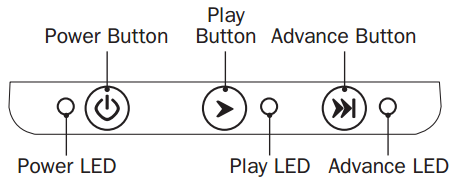
\includegraphics[width=0.8\textwidth]{img/3button.png}
	    \caption{Three Buttons Found Under Strainer}
	\end{figure}

\section{Normal Operation}
The following outlines how to get \mykbspace operating normally.

\subsection{Laptop Server and Twitter Feed}
\begin{enumerate}
	\item With the Laptop logged in, open up Visual Studio from the desktop shortcut and hit \texttt{F5}. A black Console window will open up. Refer to Figure \ref{normalVS} for an example.
	
	\begin{figure}[h!]
		\centering
	    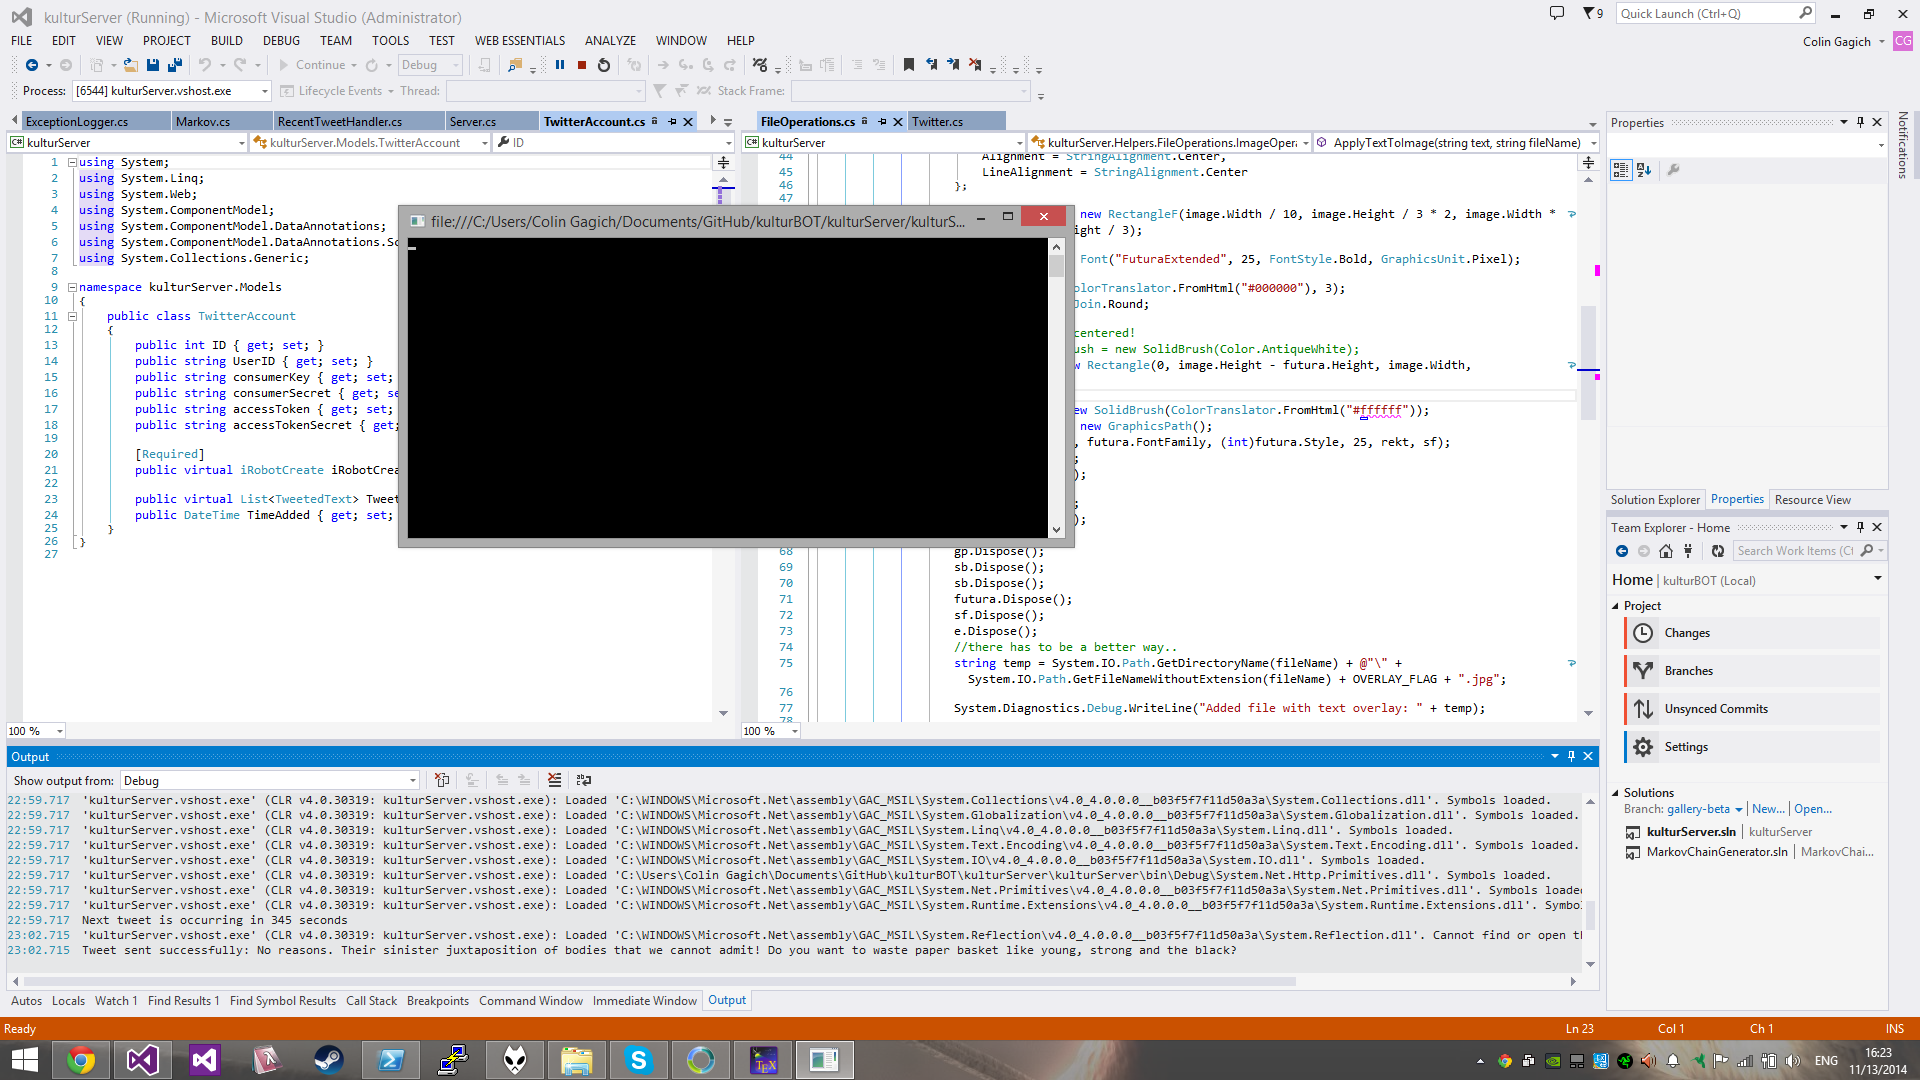
\includegraphics[width=1\textwidth]{img/normalVSlook.png}
	    \caption{Normal Operation of the Laptop}
	    \label{normalVS}
	\end{figure}
	
	\item Check the \href{https://twitter.com/kulturBOT}{\kbspace twitter feed} and ensure a tweet has been sent in the last 60 seconds. If after waiting 2 minutes no tweet appears, refer to Section \ref{kbNoTweet}. Under normal operation, no messages will appear on the black console window. If there is a problem with the internet, there will be a message in the black console window.
	
	\item To set up the live twitter feed, first connect the laptop to the projector. Ensure the projector is set up as an external display (should automatically do this). Open up Chrome from the Desktop shortcut and navigate to the \href{https://twitter.com/kulturBOT}{\kbspace twitter feed}.
\end{enumerate}
\begin{lstlisting}[frame=single]
THIS IS CODES
\end{lstlisting}

\section{Troubleshooting}
\subsection{\kbspace isn't tweeting!}
\label{kbNoTweet}

\subsection{\kbspace is taking pictures but not moving.}
\subsection{\kbspace won't turn on.}
\end{document}          
